\section{Solutions}
\label{solutions}
Given the causes of race conditions, the global solution is any such, which prevents concurrent access to shared resources.\\
This can, however, greatly depend on the resource; for example, it may not be optimal to outright force all other threads/processes to wait until a lock on a shared resource is released (further, what happens if the lock is never released? - if improper-implementation is present, this can result in boundless-waiting, if this is present in, for example, process management in a kernel, the system will likely freeze eternally, requiring a hard-reset).\\
It may not be such that access to the shared resource is one-at-a-time (see \ref{producer_consumer} for the Producer-Consumer Problem), in which case multiple-access may be granted, up to some defined limit, in the case of producer-consumer problem this upper-limit would be the size of the buffer; in these instances it may be optimal to use a counting lock, wherein an atomic lock counter is incremented upon, e.g., another write (counting semaphore; see section \ref{CountingSemaphores}).

\subsection{Busy vs. Blocked Waiting}
Busy waiting describes a synchronisation primitive in which attempted-access to a shared resource is constant, i.e the CPU is busy constantly checking if the lock has been released.\\
Synchronisation primitives which wait-busy initially seem wasteful, since the CPU cannot be used by other processes whilst waiting, and while this is true, for some operations, such as interrupt-handlers\footnote{Wherein a synchronisation-mechanism, such as a spinlock is necessary.}, which have the highest priority (must have lowest response-time, therefore), cannot sleep, since they must run an operation as soon as the lock is released. Further, if the interrupt handler were to sleep, a context switch would be required to switch to another thread, however since interrupts do not operate on a schedule (and any queueing of interrupts, e.g. interrupting an interrupt, occurs pushing another frame onto the call-stack, each higher frame returning to the frame under), it may be such that the interrupt never executes, if sleeping were allowed, therefore.

Blocked waiting describes a synchronisation primitive in which access to a critical section is controlled by flags or other signals. This allows the thread to sleep until signalled by the thread that is currently holding the lock, at which point the thread can resume and carry out its operation in the critical section. With reference to the Producer-Consumer Problem, if the producer is filling the shared-buffer, the consumer thread can sleep (allowing it to be used by other processes) until it receives a signal from the producer indicating the producer has finished with the shared-resource (buffer), as such allowing the consumer to carry out its transfer (or other such) operation(s).

\subsection{Peterson's Solution}
Peterson's solution is one solution to synchronising concurrent-access to a shared-resource.\\
This works by two processes each having a \texttt{turn} variable, which indicates which of the two process' turn it is to enter the critical section.
Further, a two-element global-Boolean-array, \texttt{flag}, allows each process to set \texttt{True} or \texttt{False} if it wishes to enter the critical section. Initially, the \texttt{flag} array will be set to \texttt{False} for both processes.\\
From this, a busy-waiting cycle checks \texttt{turn}, and if the process whose 'turn' it is to enter the critical section has also set \texttt{True} in \texttt{flag}, that process is allowed to enter the critical section.\\
However, this relies on the process entering the critical section to set \texttt{False} in \texttt{flag} after their operation has completed via access to the critical section, thereby risking starvation.
Furthermore, this solution only works with two processes, extending this beyond two processes would even-greater increase the risk of starvation, as well as coordination issues, and general performance issues with this solution as a result of a simple flag array.\\
As such, this solution is not greatly used in modern systems-architecture.

\subsection{Atomic Variables}
Atomic variables take advantage of low-level Compare-and-Swap (CAS) operations to ensure when updating an atomic variable with a new value, the current value of the atomic variable is equal to the expected value, which is taken when first reading the atomic variable.\\
Applying this to the global-counter race-condition seen in snippet \ref{list:simple_race_condition}, if the counter was an atomic variable, when \texttt{T1} wishes to increment \texttt{counter}, it first copies the current value, let this be 0, then once it has computed the value read incremented, it stores this back in \texttt{counter}, however first checking if \texttt{counter} is equal to the expected value, which was 0, if so, no lost-updates will occur from storing the result, 1 (0 incremented), in \texttt{counter}. If, however, \texttt{counter} does \textbf{not} equal the expected value of 0, this increment must be re-calculated.\\
Clearly, this is a very inefficient solution for the counter problem shown, since given the delta (from 0) of the program's output, seen in figure \ref{fig:race_condition_output}, a significant number of re-calculations would have to occur, due to \texttt{counter} storing a value different from the first-read, expected, value. As such, with this specific example, since there is significant concurrent-access to the critical section, many CPU cycles will be wasted if using atomic variables here\footnote{It is worth mentioning that the program shown in snippet \ref{list:simple_race_condition} is slower as a result of attempted-concurrency, since there is overhead for locking mechanisms, particularly with atomic variables, in this specific example; this problem was shown to demonstrate a race-condition in the simplest case. This program should instead run on a single-thread.}.

\subsection{Mutexes}
Mutexes are a locking mechanism which implements ownership on the mutex, such that only the thread which locked the mutex can release, or unlock, it. This is in contrast to semaphores (see below), which function more-so via signalling\footnote{However, note that mutexes and \textbf{binary} semaphores are similar in kind.}.\\
One issue with mutexes as a locking mechanism is the aforementioned deadlock-situation, which can occur if there is either/or no safe sequence of processes to run, or the mutexes are improperly used, e.g. not releasing a mutex after leaving the critical section.\\
Snippet \ref{list:simple_mutex} shows a program which employs a mutex to lock access to \texttt{counter}, which results in one-million increments occurring (since \texttt{increment()} is set-up first in \texttt{thread1}), then when \texttt{decrement()} runs on \texttt{thread2} it must wait before \texttt{counterMutex} is released before it can access \texttt{counter}.

\begin{lstlisting}[language=C++, caption={Program displaying mutexes to avoid a race condition, modifying a global counter.}, label=list:simple_mutex]
#include <iostream>
#include <thread>
#include <mutex> //mutex library

int counter = 0;
std::mutex counterMutex; //setup mutex for the counter

void increment() {
    counterMutex.lock();//lock the mutex
    for (int i = 0; i < 1000000; i++) {
        counter++; //now increment 1m. times
    }
    std::cout << "Counter inside increment function: " << counter << std::endl;
    counterMutex.unlock(); //releases mutex allowing other function to access counter var. (assuming this function was run first)
}

void decrement() {
    counterMutex.lock();
    for (int i = 0; i < 1000000; i++) {
        counter--; //now decrementing 1m. times
    }
    std::cout << "Counter inside decrement function: " << counter << std::endl;
    counterMutex.unlock();
}

int main() {
    std::thread thread1(increment);
    std::thread thread2(decrement);
    
    thread1.join();
    thread2.join();
    
    std::cout << "Counter: " << counter << std::endl;
    
    return 0;
}
\end{lstlisting}

\begin{figure}[!h]
    \centering
    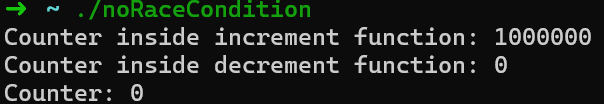
\includegraphics[scale=.5]{figures/noRaceConditionOutput.png}
    \caption{Output of program from snippet \ref{list:simple_mutex}}
    \label{fig:simple_mutex_output}
\end{figure}

The output of the program shown in snippet \ref{list:simple_mutex} can be seen in figure \ref{fig:simple_mutex_output}.


As explained in section \ref{Deadlocks}, when working with locking mechanisms, particularly mutexes, if improperly implemented, this can result in a deadlock. To demonstrate a deadlock with a slightly-modified program from that shown in snippet \ref{list:simple_mutex}, see snippet \ref{list:deadlock}.

\begin{lstlisting}[language=C++, caption={Modified version of snippet \ref{list:simple_mutex}, displaying a deadlock.}, label=list:deadlock]
#include <thread>
#include <mutex>

int counterA = 0;
std::mutex counterAMutex; //setup mutex for the counter
int counterB = 0;
std::mutex counterBMutex;

void increment() {
    counterAMutex.lock();//lock the mutex
    
    for (int i = 0; i < 1000000; i++) {
        counterA++; //now increment 1m. times
    }
    counterBMutex.lock();//wrongfully, before releasing counterAMutex, attempt to acquire counterB
    //this now depends on counterBMutex which will not be released until counterAMutex is
    counterB++; // attempting to modify counterB, though this should be unreachable due to the deadlock
    counterBMutex.unlock();
    counterAMutex.unlock(); //releases mutex allowing other function to access counter var. (assuming this function was run first)
}

void decrement() {
    counterBMutex.lock();
    for (int i = 0; i < 1000000; i++) {
        counterB--; //now decrementing 1m. times
    }
    counterAMutex.lock(); // deadlock
    counterA++;
    counterAMutex.unlock();
    counterBMutex.unlock();
}

int main() {
    std::thread thread1(increment);
    std::thread thread2(decrement);
    
    thread1.join();
    thread2.join();
    
    return 0;
}
\end{lstlisting}
In snippet \ref{list:deadlock}, due to each thread attempting to acquire each other's mutex before each has released theirs results in endless waiting; deadlock.



\subsection{Semaphores}
Semaphores are another synchronisation primitive, and have two variants: binary; and counting.
\subsubsection{Binary}
Binary semaphores have two operations \texttt{wait} and \texttt{signal}.\\
Binary semaphores are atomic variables, and either store 0 or 1, henceforth this only allows single-access to a shared-resource.\\
This is similar to Peterson's Solution, however slightly less specific, as there is no \texttt{turn} variable or \texttt{flag} array; semaphores operate via \texttt{wait} and \texttt{signal} signals, as such allows multiple processes to wait, then wake-up when they are signalled (once the critical section is free). Depending on the implementation of the binary semaphore, the queuing may be some algorithm such as FCFS, potentially allowing a priority to be specified (perhaps then implementing ageing\footnote{Increasing a process' priority the longer it waits.} to prevent total-starvation).
\subsubsection{Counting}
\label{CountingSemaphores}
All previous synchronisation primitives discussed thus-far have only allowed one process to hold a shared-resource at a time, however, counting semaphores, by contrast, can allow multiple processes to hold the same resource. This may seem as though race conditions are guaranteed if using counting semaphores, however, it is for this reason that this synchronisation method is only applicable to particular tasks.\\
With reference to the Producer-Consumer Problem, the counting semaphore may store the filled slots in the buffer, such that the producer increments the semaphore upon adding an item to the buffer, with the consumer decrementing the semaphore upon transferring-out an item from the buffer. Note that data may still be overwritten in the buffer, as such a mutex is required for accessing the shared buffer, with a second semaphore being to track the number of empty slots. This is more efficient than only using a mutex, since else both the producer and consumer would have to acquire the mutex in order to check if the buffer is full/empty, respectively for the producer and the consumer. In this way, busy-waiting is avoided, since one of the threads can sleep until signalled by the other, then acquiring the mutex and producing or consuming items to/from the buffer. As a result of blocked-waiting, this scales significantly-better (having many producers and consumers) than using only a mutex on the critical section. (\cite{geeksSemaphore}).
